% !tex root = ../main.tex

\section{Some Common Elements}
\label{sec:CommonElements}

\subsection{Sections and Subsections}
Enumeration of section headings is desirable, but not required. When numbered, please be consistent throughout the article, that is, all headings and all levels of section headings in the article should be enumerated. Primary headings are designated with Roman numerals, secondary with capital letters, tertiary with Arabic numbers; and quaternary with lowercase letters. Reference and Acknowledgment headings are unlike all other section headings in text. They are never enumerated. They are simply primary headings without labels, regardless of whether the other headings in the article are enumerated. 

\subsection{Citations to the Bibliography}
The coding for the citations is made with the \LaTeX\ $\backslash${\tt{cite}} command. 
This will display as: see \cite{RPS}.

For multiple citations code as follows: {\tt{$\backslash$cite\{ref1,ref2,ref3\}}}
 which will produce \cite{RPS}. For reference ranges that are not consecutive code as {\tt{$\backslash$cite\{ref1,ref2,ref3,ref9\}}} which will produce  \cite{RPS}

\subsection{Lists}
In this section, we will consider three types of lists: simple unnumbered, numbered, and bulleted. There have been many options added to IEEEtran to enhance the creation of lists. If your lists are more complex than those shown below, please refer to the original ``IEEEtran\_HOWTO.pdf'' for additional options.\\

\subsubsection*{\bf A plain  unnumbered list}
\begin{list}{}{}
\item{bare\_jrnl.tex}
\item{bare\_conf.tex}
\item{bare\_jrnl\_compsoc.tex}
\item{bare\_conf\_compsoc.tex}
\item{bare\_jrnl\_comsoc.tex}
\end{list}

\subsubsection*{\bf A simple numbered list}
\begin{enumerate}
\item{bare\_jrnl.tex}
\item{bare\_conf.tex}
\item{bare\_jrnl\_compsoc.tex}
\item{bare\_conf\_compsoc.tex}
\item{bare\_jrnl\_comsoc.tex}
\end{enumerate}

\subsubsection*{\bf A simple bulleted list}
\begin{itemize}
\item{bare\_jrnl.tex}
\item{bare\_conf.tex}
\item{bare\_jrnl\_compsoc.tex}
\item{bare\_conf\_compsoc.tex}
\item{bare\_jrnl\_comsoc.tex}
\end{itemize}





\subsection{Figures}
\cref{fig_1} is an example of a floating figure using the graphicx package.
Note that $\backslash${\tt{label}} must occur AFTER (or within) $\backslash${\tt{caption}}.
For figures, $\backslash${\tt{caption}} should occur after the $\backslash${\tt{includegraphics}}.

\begin{figure}[!t]
\centering
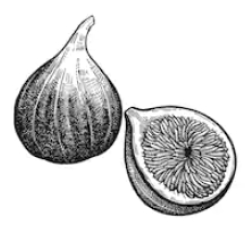
\includegraphics[width=2.5in]{fig/fig1}
\caption{Simulation results for the network.}
\label{fig_1}
\end{figure}

\cref{fig_first_case} and \cref{fig_second_case} is an example of a double column floating figure using two subfigures.
 (The subfig.sty package must be loaded for this to work.)
 The subfigure $\backslash${\tt{label}} commands are set within each subfloat command,
 and the $\backslash${\tt{label}} for the overall figure must come after $\backslash${\tt{caption}}.
 $\backslash${\tt{hfil}} is used as a separator to get equal spacing.
 The combined width of all the parts of the figure should do not exceed the text width or a line break will occur.
%
\begin{figure*}[!t]
\centering
\subfloat[]{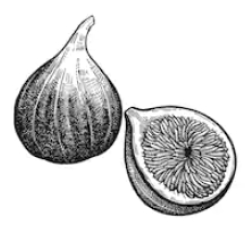
\includegraphics[width=2.5in]{fig/fig1}%
\label{fig_first_case}}
\hfil
\subfloat[]{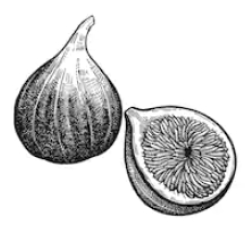
\includegraphics[width=2.5in]{fig/fig1}%
\label{fig_second_case}}
\caption{Dae. Ad quatur autat ut porepel itemoles dolor autem fuga. Bus quia con nessunti as remo di quatus non perum que nimus. (a) Case I. (b) Case II.}
\label{fig_sim}
\end{figure*}

Note that often IEEE papers with multi-part figures do not place the labels within the image itself (using the optional argument to $\backslash${\tt{subfloat}}[]), but instead will
reference/describe all of them (a), (b), etc., within the main caption.
Be aware that for subfig.sty to generate the (a), (b), etc., subfigure
labels, the optional argument to $\backslash${\tt{subfloat}} must be present. If a
subcaption is not desired, leave its contents blank,
e.g.,$\backslash${\tt{subfloat}}[].


\subsection{Tables}
Note that, for IEEE-style tables, the
 $\backslash${\tt{caption}} command should come BEFORE the table. Table captions use title case. Articles (a, an, the), coordinating conjunctions (and, but, for, or, nor), and most short prepositions are lowercase unless they are the first or last word. Table text will default to $\backslash${\tt{footnotesize}} as
 the IEEE normally uses this smaller font for tables.
 The $\backslash${\tt{label}} must come after $\backslash${\tt{caption}} as always.
 
\begin{table}[!t]
\caption{An Example of a Table\label{tab:table1}}
\centering
\begin{tabular}{|c||c|}
\hline
One & Two\\
\hline
Three & Four\\
\hline
\end{tabular}
\end{table}


\subsection{Algorithms}
Algorithms should be numbered and include a short title. They are set off from the text with rules above and below the title and after the last line.

\begin{algorithm}[H]
\caption{Weighted Tanimoto ELM.}\label{alg:alg1}
\begin{algorithmic}
\STATE 
\STATE {\textsc{TRAIN}}$(\mathbf{X} \mathbf{T})$
\STATE \hspace{0.5cm}$ \textbf{select randomly } W \subset \mathbf{X}  $
\STATE \hspace{0.5cm}$ N_\mathbf{t} \gets | \{ i : \mathbf{t}_i = \mathbf{t} \} | $ \textbf{ for } $ \mathbf{t}= -1,+1 $
\STATE \hspace{0.5cm}$ B_i \gets \sqrt{ \textsc{max}(N_{-1},N_{+1}) / N_{\mathbf{t}_i} } $ \textbf{ for } $ i = 1,...,N $
\STATE \hspace{0.5cm}$ \hat{\mathbf{H}} \gets  B \cdot (\mathbf{X}^T\textbf{W})/( \mathbb{1}\mathbf{X} + \mathbb{1}\textbf{W} - \mathbf{X}^T\textbf{W} ) $
\STATE \hspace{0.5cm}$ \beta \gets \left ( I/C + \hat{\mathbf{H}}^T\hat{\mathbf{H}} \right )^{-1}(\hat{\mathbf{H}}^T B\cdot \mathbf{T})  $
\STATE \hspace{0.5cm}\textbf{return}  $\textbf{W},  \beta $
\STATE 
\STATE {\textsc{PREDICT}}$(\mathbf{X} )$
\STATE \hspace{0.5cm}$ \mathbf{H} \gets  (\mathbf{X}^T\textbf{W} )/( \mathbb{1}\mathbf{X}  + \mathbb{1}\textbf{W}- \mathbf{X}^T\textbf{W}  ) $
\STATE \hspace{0.5cm}\textbf{return}  $\textsc{sign}( \mathbf{H} \beta )$
\end{algorithmic}
\label{alg1}
\end{algorithm}

Que sunt eum lam eos si dic to estist, culluptium quid qui nestrum nobis reiumquiatur minimus minctem. Ro moluptat fuga. Itatquiam ut laborpo rersped exceres vollandi repudaerem. Ulparci sunt, qui doluptaquis sumquia ndestiu sapient iorepella sunti veribus. Ro moluptat fuga. Itatquiam ut laborpo rersped exceres vollandi repudaerem. 